\documentclass[11pt,]{article}
\usepackage[left=1in,top=1in,right=1in,bottom=1in]{geometry}
\newcommand*{\authorfont}{\fontfamily{phv}\selectfont}
\usepackage[]{mathpazo}


  \usepackage[T1]{fontenc}
  \usepackage[utf8]{inputenc}




\usepackage{abstract}
\renewcommand{\abstractname}{}    % clear the title
\renewcommand{\absnamepos}{empty} % originally center

\renewenvironment{abstract}
 {{%
    \setlength{\leftmargin}{0mm}
    \setlength{\rightmargin}{\leftmargin}%
  }%
  \relax}
 {\endlist}

\makeatletter
\def\@maketitle{%
  \newpage
%  \null
%  \vskip 2em%
%  \begin{center}%
  \let \footnote \thanks
    {\fontsize{18}{20}\selectfont\raggedright  \setlength{\parindent}{0pt} \@title \par}%
}
%\fi
\makeatother




\setcounter{secnumdepth}{0}

\usepackage{color}
\usepackage{fancyvrb}
\newcommand{\VerbBar}{|}
\newcommand{\VERB}{\Verb[commandchars=\\\{\}]}
\DefineVerbatimEnvironment{Highlighting}{Verbatim}{commandchars=\\\{\}}
% Add ',fontsize=\small' for more characters per line
\usepackage{framed}
\definecolor{shadecolor}{RGB}{248,248,248}
\newenvironment{Shaded}{\begin{snugshade}}{\end{snugshade}}
\newcommand{\AlertTok}[1]{\textcolor[rgb]{0.94,0.16,0.16}{#1}}
\newcommand{\AnnotationTok}[1]{\textcolor[rgb]{0.56,0.35,0.01}{\textbf{\textit{#1}}}}
\newcommand{\AttributeTok}[1]{\textcolor[rgb]{0.77,0.63,0.00}{#1}}
\newcommand{\BaseNTok}[1]{\textcolor[rgb]{0.00,0.00,0.81}{#1}}
\newcommand{\BuiltInTok}[1]{#1}
\newcommand{\CharTok}[1]{\textcolor[rgb]{0.31,0.60,0.02}{#1}}
\newcommand{\CommentTok}[1]{\textcolor[rgb]{0.56,0.35,0.01}{\textit{#1}}}
\newcommand{\CommentVarTok}[1]{\textcolor[rgb]{0.56,0.35,0.01}{\textbf{\textit{#1}}}}
\newcommand{\ConstantTok}[1]{\textcolor[rgb]{0.00,0.00,0.00}{#1}}
\newcommand{\ControlFlowTok}[1]{\textcolor[rgb]{0.13,0.29,0.53}{\textbf{#1}}}
\newcommand{\DataTypeTok}[1]{\textcolor[rgb]{0.13,0.29,0.53}{#1}}
\newcommand{\DecValTok}[1]{\textcolor[rgb]{0.00,0.00,0.81}{#1}}
\newcommand{\DocumentationTok}[1]{\textcolor[rgb]{0.56,0.35,0.01}{\textbf{\textit{#1}}}}
\newcommand{\ErrorTok}[1]{\textcolor[rgb]{0.64,0.00,0.00}{\textbf{#1}}}
\newcommand{\ExtensionTok}[1]{#1}
\newcommand{\FloatTok}[1]{\textcolor[rgb]{0.00,0.00,0.81}{#1}}
\newcommand{\FunctionTok}[1]{\textcolor[rgb]{0.00,0.00,0.00}{#1}}
\newcommand{\ImportTok}[1]{#1}
\newcommand{\InformationTok}[1]{\textcolor[rgb]{0.56,0.35,0.01}{\textbf{\textit{#1}}}}
\newcommand{\KeywordTok}[1]{\textcolor[rgb]{0.13,0.29,0.53}{\textbf{#1}}}
\newcommand{\NormalTok}[1]{#1}
\newcommand{\OperatorTok}[1]{\textcolor[rgb]{0.81,0.36,0.00}{\textbf{#1}}}
\newcommand{\OtherTok}[1]{\textcolor[rgb]{0.56,0.35,0.01}{#1}}
\newcommand{\PreprocessorTok}[1]{\textcolor[rgb]{0.56,0.35,0.01}{\textit{#1}}}
\newcommand{\RegionMarkerTok}[1]{#1}
\newcommand{\SpecialCharTok}[1]{\textcolor[rgb]{0.00,0.00,0.00}{#1}}
\newcommand{\SpecialStringTok}[1]{\textcolor[rgb]{0.31,0.60,0.02}{#1}}
\newcommand{\StringTok}[1]{\textcolor[rgb]{0.31,0.60,0.02}{#1}}
\newcommand{\VariableTok}[1]{\textcolor[rgb]{0.00,0.00,0.00}{#1}}
\newcommand{\VerbatimStringTok}[1]{\textcolor[rgb]{0.31,0.60,0.02}{#1}}
\newcommand{\WarningTok}[1]{\textcolor[rgb]{0.56,0.35,0.01}{\textbf{\textit{#1}}}}
\usepackage{longtable,booktabs}

\usepackage{graphicx,grffile}
\makeatletter
\def\maxwidth{\ifdim\Gin@nat@width>\linewidth\linewidth\else\Gin@nat@width\fi}
\def\maxheight{\ifdim\Gin@nat@height>\textheight\textheight\else\Gin@nat@height\fi}
\makeatother
% Scale images if necessary, so that they will not overflow the page
% margins by default, and it is still possible to overwrite the defaults
% using explicit options in \includegraphics[width, height, ...]{}
\setkeys{Gin}{width=\maxwidth,height=\maxheight,keepaspectratio}


\title{Application of Machine Learning on Fundamental Stock Price Analysis  }



\author{\Large Albina Cako, BSc\vspace{0.05in} \newline\normalsize\emph{York University, Certificate in Machine Learning}   \and \Large Colin Green, BSc\vspace{0.05in} \newline\normalsize\emph{York University, Certificate in Machine Learning}   \and \Large Lucy Zhang, BSc\vspace{0.05in} \newline\normalsize\emph{York University, Certificate in Machine Learning}   \and \Large Sean X. Zhang, MSc\vspace{0.05in} \newline\normalsize\emph{York University, Certificate in Machine Learning}  }


\date{}

\usepackage{titlesec}

\titleformat*{\section}{\normalsize\bfseries}
\titleformat*{\subsection}{\normalsize\itshape}
\titleformat*{\subsubsection}{\normalsize\itshape}
\titleformat*{\paragraph}{\normalsize\itshape}
\titleformat*{\subparagraph}{\normalsize\itshape}





\newtheorem{hypothesis}{Hypothesis}
\usepackage{setspace}


% set default figure placement to htbp
\makeatletter
\def\fps@figure{htbp}
\makeatother

\usepackage{hyperref}
\usepackage{graphicx}
\usepackage{subfig}

% move the hyperref stuff down here, after header-includes, to allow for - \usepackage{hyperref}

\makeatletter
\@ifpackageloaded{hyperref}{}{%
\ifxetex
  \PassOptionsToPackage{hyphens}{url}\usepackage[setpagesize=false, % page size defined by xetex
              unicode=false, % unicode breaks when used with xetex
              xetex]{hyperref}
\else
  \PassOptionsToPackage{hyphens}{url}\usepackage[draft,unicode=true]{hyperref}
\fi
}

\@ifpackageloaded{color}{
    \PassOptionsToPackage{usenames,dvipsnames}{color}
}{%
    \usepackage[usenames,dvipsnames]{color}
}
\makeatother
\hypersetup{breaklinks=true,
            bookmarks=true,
            pdfauthor={Albina Cako, BSc (York University, Certificate in Machine Learning) and Colin Green, BSc (York University, Certificate in Machine Learning) and Lucy Zhang, BSc (York University, Certificate in Machine Learning) and Sean X. Zhang, MSc (York University, Certificate in Machine Learning)},
             pdfkeywords = {stock price, fundamental analysis, machine learning, R},  
            pdftitle={Application of Machine Learning on Fundamental Stock Price Analysis},
            colorlinks=true,
            citecolor=blue,
            urlcolor=blue,
            linkcolor=magenta,
            pdfborder={0 0 0}}
\urlstyle{same}  % don't use monospace font for urls

% Add an option for endnotes. -----


% add tightlist ----------
\providecommand{\tightlist}{%
\setlength{\itemsep}{0pt}\setlength{\parskip}{0pt}}

% add some other packages ----------

% \usepackage{multicol}
% This should regulate where figures float
% See: https://tex.stackexchange.com/questions/2275/keeping-tables-figures-close-to-where-they-are-mentioned
\usepackage[section]{placeins}


\begin{document}
	
% \pagenumbering{arabic}% resets `page` counter to 1 
%
% \maketitle

{% \usefont{T1}{pnc}{m}{n}
\setlength{\parindent}{0pt}
\thispagestyle{plain}
{\fontsize{18}{20}\selectfont\raggedright 
\maketitle  % title \par  

}

{
   \vskip 13.5pt\relax \normalsize\fontsize{11}{12} 
\textbf{\authorfont Albina Cako, BSc} \hskip 15pt \emph{\small York University, Certificate in Machine Learning}   \par \textbf{\authorfont Colin Green, BSc} \hskip 15pt \emph{\small York University, Certificate in Machine Learning}   \par \textbf{\authorfont Lucy Zhang, BSc} \hskip 15pt \emph{\small York University, Certificate in Machine Learning}   \par \textbf{\authorfont Sean X. Zhang, MSc} \hskip 15pt \emph{\small York University, Certificate in Machine Learning}   

}

}








\begin{abstract}

    \hbox{\vrule height .2pt width 39.14pc}

    \vskip 8.5pt % \small 

\noindent Abstract:


\vskip 8.5pt \noindent \emph{Keywords}: stock price, fundamental analysis, machine learning, R \par

    \hbox{\vrule height .2pt width 39.14pc}



\end{abstract}


\vskip -8.5pt


 % removetitleabstract

\noindent  

\hypertarget{introduction}{%
\section{Introduction}\label{introduction}}

\hypertarget{background}{%
\subsection{Background}\label{background}}

The stock market is a marketplace where investors can purchase or sell
shares of publicly traded companies. As of 2019, the amount of money
invested in the global stock market has surpassed over \$85 trillion.
Since the inception of the stock market, investors have continuously
sought to develop methods of improving their returns. Currently, there
are two main schools of thought when it comes to stock market analysis:
technical analysis and fundamental analysis.

\emph{Technical analysis} looks at buying and selling trends of a
particular stock. The core theory of technical analysis assumes that all
information is already factored into the stock price. As such, technical
analysis prioritizes identifying patterns or trends in time-series data
to predict stock price at a particular time point.

\emph{Fundamental analysis} attempts to measure the intrinsic value of a
company by studying information from that company's balance sheet, such
as revenue or debt. Fundamental analysis attempts to identify companies
that appear to be `undervalued' or `overvalued' to inform buy or sell
recommendations.

Previous machine learning models that simulated stock market returns
have largely focused on using time series data to predict stock trends,
which is more akin to technical analysis. However, such models have run
into challenges such as overfitting or a lack of interpretability. One
benefit of fundamental analysis is that it allows the investor to learn
about which aspects of a company's financials will influence that
company's stock price; it is more interpretable. As there are dozens to
hundreds of variables on a company's balance sheet, the use of
machine-learning approaches may augment fundamental analysis by
pinpointing important markers of a company's financials and their
relationship with the stock price.

\hypertarget{objective}{%
\subsection{Objective}\label{objective}}

In this project, we apply machine learning and data science techniques
to predict the market capitalization, which is how much company is worth
on the stock market. Stock price can then be calculated by dividing
market capitalization by total number of stocks issued. We also create
an application using R shiny to be used as a guide for investors. This
application would be used individuals interested in checking their stock
analyses with a machine learning prediction. The application could be
used by financial analysts, portfolio managers, or non-professional
investors with an interest in fundamental analysis.

\hypertarget{methodology}{%
\section{Methodology}\label{methodology}}

\hypertarget{data-preprocessing}{%
\subsection{Data Preprocessing}\label{data-preprocessing}}

\hypertarget{missing-values}{%
\subsection{Missing Values}\label{missing-values}}

\hypertarget{data-curation}{%
\subsection{Data Curation}\label{data-curation}}

\hypertarget{modeling}{%
\subsection{Modeling}\label{modeling}}

\hypertarget{feature-selection}{%
\subsection{Feature Selection}\label{feature-selection}}

Talk about the decision tree here

\hypertarget{principle-component-analysis}{%
\subsection{Principle Component
Analysis}\label{principle-component-analysis}}

We applied Principle Component Analysis (PCA) to our feature dataset for
dimensionality reduction before unsupervised learning with k-Nearest
Neighbor (kNN). PCA creates orthoganal `principle components' of the
feature set, reducing multicollinearity within the data. While k-NN is
non-parametric, reducing multicollinearity before performing k-NN could
lead to greater discrimination in-between points.

\hypertarget{unsupervised-learning}{%
\subsection{Unsupervised Learning}\label{unsupervised-learning}}

The k-NN algorithm was run to cluster the data before supervised
learning. The number of clusters was evaluated by plotting the
within-cluster sum of squares (WSS) against the number of clusters (k).
The optimal number of clusters was chosen based on a combination of the
`elbow method' and domain knowledge.

\hypertarget{supervised-learning}{%
\subsection{Supervised Learning}\label{supervised-learning}}

\hypertarget{deployment}{%
\subsection{Deployment}\label{deployment}}

\hypertarget{results}{%
\section{Results}\label{results}}

\hypertarget{data-exploration}{%
\subsection{Data Exploration}\label{data-exploration}}

\#\#\#Data Preparation The original data is from Kaggle and have several
different CSV files include the stock information for different years.
We combined the CSV files into one full data set for our project

\begin{Shaded}
\begin{Highlighting}[]
\CommentTok{#load in the first file}
\NormalTok{data_}\DecValTok{2014}\NormalTok{ <-}\StringTok{ }\KeywordTok{read.csv}\NormalTok{(}\StringTok{'2014_Financial_Data.csv'}\NormalTok{)}
\NormalTok{data_}\DecValTok{2015}\NormalTok{ <-}\StringTok{ }\KeywordTok{read.csv}\NormalTok{(}\StringTok{'2015_Financial_Data.csv'}\NormalTok{)}
\NormalTok{data_}\DecValTok{2016}\NormalTok{ <-}\StringTok{ }\KeywordTok{read.csv}\NormalTok{(}\StringTok{'2016_Financial_Data.csv'}\NormalTok{)}
\NormalTok{data_}\DecValTok{2017}\NormalTok{ <-}\StringTok{ }\KeywordTok{read.csv}\NormalTok{(}\StringTok{'2017_Financial_Data.csv'}\NormalTok{)}
\NormalTok{data_}\DecValTok{2018}\NormalTok{ <-}\StringTok{ }\KeywordTok{read.csv}\NormalTok{(}\StringTok{'2018_Financial_Data.csv'}\NormalTok{)}

\CommentTok{#add a column for year}
\NormalTok{data_}\DecValTok{2014}\NormalTok{ <-}\StringTok{ }\NormalTok{data_}\DecValTok{2014} \OperatorTok\StringTok{ }\KeywordTok{mutate}\NormalTok{(}\DataTypeTok{year=}\DecValTok{2014}\NormalTok{)}
\NormalTok{data_}\DecValTok{2015}\NormalTok{ <-}\StringTok{ }\NormalTok{data_}\DecValTok{2015} \OperatorTok\StringTok{ }\KeywordTok{mutate}\NormalTok{(}\DataTypeTok{year=}\DecValTok{2015}\NormalTok{)}
\NormalTok{data_}\DecValTok{2016}\NormalTok{ <-}\StringTok{ }\NormalTok{data_}\DecValTok{2016} \OperatorTok\StringTok{ }\KeywordTok{mutate}\NormalTok{(}\DataTypeTok{year=}\DecValTok{2016}\NormalTok{)}
\NormalTok{data_}\DecValTok{2017}\NormalTok{ <-}\StringTok{ }\NormalTok{data_}\DecValTok{2017} \OperatorTok\StringTok{ }\KeywordTok{mutate}\NormalTok{(}\DataTypeTok{year=}\DecValTok{2017}\NormalTok{)}
\NormalTok{data_}\DecValTok{2018}\NormalTok{ <-}\StringTok{ }\NormalTok{data_}\DecValTok{2018} \OperatorTok\StringTok{ }\KeywordTok{mutate}\NormalTok{(}\DataTypeTok{year=}\DecValTok{2018}\NormalTok{)}

\CommentTok{#fix the column name}
\KeywordTok{colnames}\NormalTok{(data_}\DecValTok{2014}\NormalTok{)[}\DecValTok{224}\NormalTok{] <-}\StringTok{ 'PRICE.VARR'}
\KeywordTok{colnames}\NormalTok{(data_}\DecValTok{2015}\NormalTok{)[}\DecValTok{224}\NormalTok{] <-}\StringTok{ 'PRICE.VARR'}
\KeywordTok{colnames}\NormalTok{(data_}\DecValTok{2016}\NormalTok{)[}\DecValTok{224}\NormalTok{] <-}\StringTok{ 'PRICE.VARR'}
\KeywordTok{colnames}\NormalTok{(data_}\DecValTok{2017}\NormalTok{)[}\DecValTok{224}\NormalTok{] <-}\StringTok{ 'PRICE.VARR'}
\KeywordTok{colnames}\NormalTok{(data_}\DecValTok{2018}\NormalTok{)[}\DecValTok{224}\NormalTok{] <-}\StringTok{ 'PRICE.VARR'}

\NormalTok{complete_data <-}\StringTok{ }\KeywordTok{rbind}\NormalTok{(data_}\DecValTok{2014}\NormalTok{, data_}\DecValTok{2015}\NormalTok{, data_}\DecValTok{2016}\NormalTok{, data_}\DecValTok{2017}\NormalTok{, data_}\DecValTok{2018}\NormalTok{)}

\CommentTok{#only include fundamental columns}
\NormalTok{complete_data <-}\StringTok{ }\KeywordTok{subset}\NormalTok{(complete_data[,}\KeywordTok{c}\NormalTok{(}\DecValTok{1}\OperatorTok{:}\DecValTok{4}\NormalTok{,}\DecValTok{6}\OperatorTok{:}\DecValTok{8}\NormalTok{,}\DecValTok{10}\NormalTok{,}\DecValTok{12}\OperatorTok{:}\DecValTok{14}\NormalTok{,}\DecValTok{16}\NormalTok{,}\DecValTok{20}\NormalTok{,}\DecValTok{22}\NormalTok{,}\DecValTok{30}\NormalTok{,}\DecValTok{33}\NormalTok{,}\DecValTok{34}\NormalTok{,}\DecValTok{36}\NormalTok{,}\DecValTok{38}\NormalTok{,}\DecValTok{40}\OperatorTok{:}\DecValTok{43}\NormalTok{,}\DecValTok{45}\OperatorTok{:}\DecValTok{53}\NormalTok{,}\DecValTok{55}\NormalTok{,}\DecValTok{56}\NormalTok{,}\DecValTok{60}\OperatorTok{:}\DecValTok{74}\NormalTok{,}\DecValTok{142}\NormalTok{,}\DecValTok{176}\NormalTok{,}\DecValTok{179}\OperatorTok{:}\DecValTok{190}\NormalTok{,}\DecValTok{223}\NormalTok{,}\DecValTok{226}\NormalTok{)])}
\NormalTok{complete_data <-}\StringTok{ }\NormalTok{complete_data[complete_data}\OperatorTok{$}\NormalTok{X }\OperatorTok{!=}\StringTok{ 'IGLD'}\NormalTok{, ]}
\NormalTok{complete_data <-}\StringTok{ }\NormalTok{complete_data[complete_data}\OperatorTok{$}\NormalTok{X }\OperatorTok{!=}\StringTok{ 'SBT'}\NormalTok{, ]}
\NormalTok{complete_data <-}\StringTok{ }\NormalTok{complete_data[complete_data}\OperatorTok{$}\NormalTok{X }\OperatorTok{!=}\StringTok{ 'KST'}\NormalTok{, ]}
\NormalTok{complete_data <-}\StringTok{ }\NormalTok{complete_data[complete_data}\OperatorTok{$}\NormalTok{X }\OperatorTok{!=}\StringTok{ 'AMX'}\NormalTok{, ]}
\end{Highlighting}
\end{Shaded}

After we finished the first step of data cleaning, we want to do the
data validation. For missing values, as the plot shown, a lot of
observations make up the majority of the missing data and we decided to
remove observations that have more than a third of the columns NA.After
we removed those observations, we set the sector and year columns as a
factor and saved the new data set into a new CSV files for futhur data
exploration.

\begin{Shaded}
\begin{Highlighting}[]
\KeywordTok{missing_plot}\NormalTok{(complete_data)}
\end{Highlighting}
\end{Shaded}

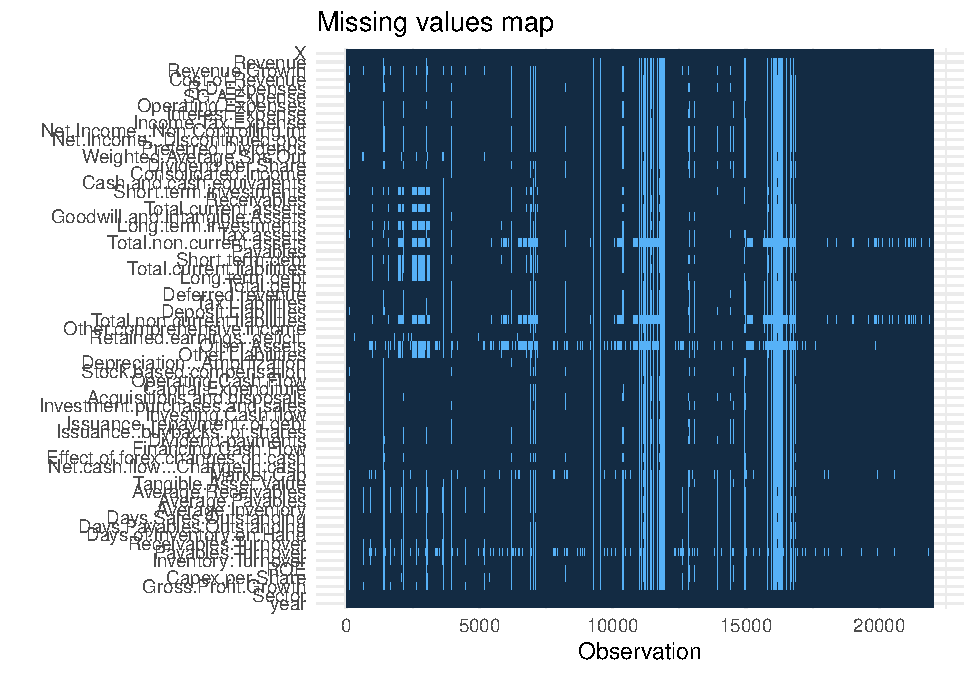
\includegraphics{stock_analysis_files/figure-latex/unnamed-chunk-2-1.pdf}

\begin{Shaded}
\begin{Highlighting}[]
\CommentTok{#sort((sapply(complete_data, function(x) sum(is.na(x)))), decreasing=TRUE)}

\NormalTok{complete_data_remove<-complete_data[}\KeywordTok{which}\NormalTok{(}\KeywordTok{rowMeans}\NormalTok{(}\OperatorTok{!}\KeywordTok{is.na}\NormalTok{(complete_data))}\OperatorTok{>}\NormalTok{(}\DecValTok{1}\OperatorTok{/}\DecValTok{3}\NormalTok{)),]}
\KeywordTok{missing_plot}\NormalTok{(complete_data_remove)}
\end{Highlighting}
\end{Shaded}

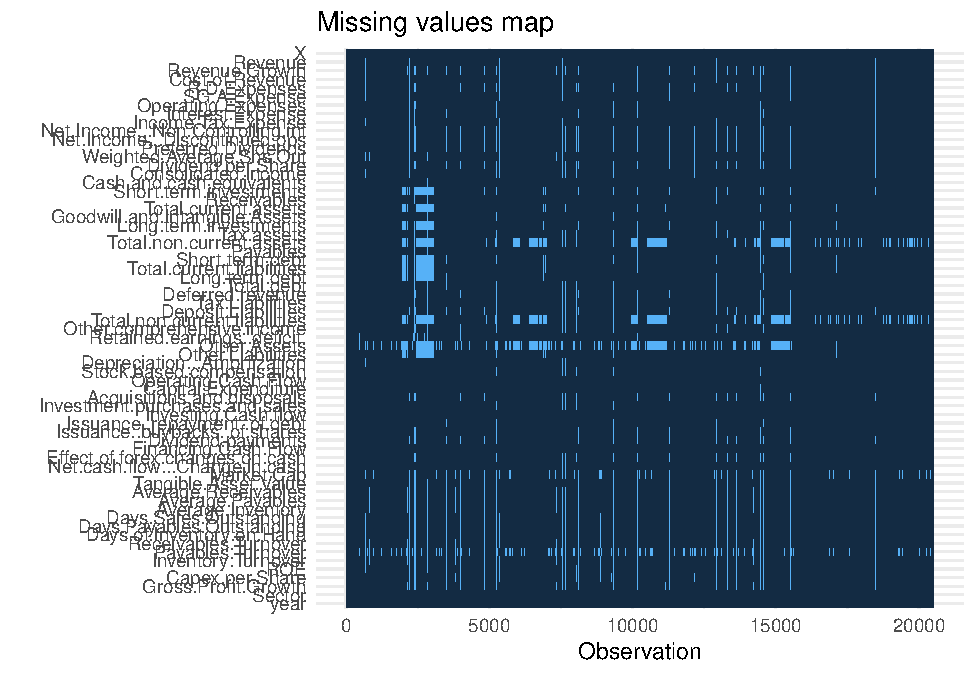
\includegraphics{stock_analysis_files/figure-latex/unnamed-chunk-2-2.pdf}

\begin{Shaded}
\begin{Highlighting}[]
\CommentTok{#sort((sapply(complete_data_remove, function(x) sum(is.na(x)))), decreasing=TRUE)}

\NormalTok{complete_data_remove}\OperatorTok{$}\NormalTok{Sector <-}\StringTok{ }\KeywordTok{as.factor}\NormalTok{(complete_data_remove}\OperatorTok{$}\NormalTok{Sector)}
\NormalTok{complete_data_remove}\OperatorTok{$}\NormalTok{year <-}\StringTok{ }\KeywordTok{as.factor}\NormalTok{(complete_data_remove}\OperatorTok{$}\NormalTok{year)}

\CommentTok{#save the new data set as a csv}
\CommentTok{#write.csv(complete_data_remove,"fundamental_data.csv")}
\NormalTok{pvq <-}\StringTok{ }\KeywordTok{quantile}\NormalTok{(complete_data_remove}\OperatorTok{$}\NormalTok{Market.Cap, }\DataTypeTok{probs =} \KeywordTok{c}\NormalTok{(}\FloatTok{0.01}\NormalTok{,}\FloatTok{0.99}\NormalTok{), }\DataTypeTok{names=}\OtherTok{FALSE}\NormalTok{, }\DataTypeTok{na.rm=}\OtherTok{TRUE}\NormalTok{)}
\NormalTok{plot_data <-}\StringTok{ }\NormalTok{complete_data_remove}
\NormalTok{plot_data[plot_data}\OperatorTok{==}\DecValTok{0}\NormalTok{] <-}\StringTok{ }\OtherTok{NA}
\end{Highlighting}
\end{Shaded}

To account for missing values, we chose to use the CART (Classification
and Regression Trees) method of imputation
(\hyperref[sec:fig2]{Figure 2}). Blue represents the distribution of the
original data, while red represents the distribution of imputed data.
After the imputation there are still 4 columns has missing values.

\begin{verbatim}
##       X                Revenue           Revenue.Growth    
##  Length:20526       Min.   :-6.276e+08   Min.   :   -6.87  
##  Class :character   1st Qu.: 6.567e+07   1st Qu.:   -0.01  
##  Mode  :character   Median : 4.684e+08   Median :    0.06  
##                     Mean   : 4.883e+09   Mean   :    5.72  
##                     3rd Qu.: 2.367e+09   3rd Qu.:    0.18  
##                     Max.   : 5.003e+11   Max.   :42138.66  
##  Cost.of.Revenue       R.D.Expenses         SG.A.Expense       
##  Min.   :-2.987e+09   Min.   :-1.098e+08   Min.   :-1.402e+08  
##  1st Qu.: 3.380e+06   1st Qu.: 0.000e+00   1st Qu.: 1.778e+07  
##  Median : 1.519e+08   Median : 0.000e+00   Median : 8.048e+07  
##  Mean   : 2.942e+09   Mean   : 1.037e+08   Mean   : 8.508e+08  
##  3rd Qu.: 1.171e+09   3rd Qu.: 1.235e+07   3rd Qu.: 3.698e+08  
##  Max.   : 3.771e+11   Max.   : 2.884e+10   Max.   : 1.065e+11  
##  Operating.Expenses   Interest.Expense     Income.Tax.Expense  
##  Min.   :-5.496e+09   Min.   :-1.711e+09   Min.   :-7.380e+11  
##  1st Qu.: 3.582e+07   1st Qu.: 0.000e+00   1st Qu.: 0.000e+00  
##  Median : 1.565e+08   Median : 3.684e+06   Median : 3.374e+06  
##  Mean   : 1.354e+09   Mean   : 9.349e+07   Mean   : 1.242e+08  
##  3rd Qu.: 6.233e+08   3rd Qu.: 4.994e+07   3rd Qu.: 4.443e+07  
##  Max.   : 1.065e+11   Max.   : 1.845e+10   Max.   : 8.490e+11  
##  Net.Income...Non.Controlling.int Net.Income...Discontinued.ops
##  Min.   :-1.587e+09               Min.   :-1.591e+10           
##  1st Qu.: 0.000e+00               1st Qu.: 0.000e+00           
##  Median : 0.000e+00               Median : 0.000e+00           
##  Mean   : 1.343e+07               Mean   :-4.430e+06           
##  3rd Qu.: 0.000e+00               3rd Qu.: 0.000e+00           
##  Max.   : 6.431e+09               Max.   : 8.368e+09           
##  Preferred.Dividends  Weighted.Average.Shs.Out Dividend.per.Share 
##  Min.   :-161000000   Min.   :0.000e+00        Min.   :    0.000  
##  1st Qu.:         0   1st Qu.:1.743e+07        1st Qu.:    0.000  
##  Median :         0   Median :4.421e+07        Median :    0.000  
##  Mean   :   4816894   Mean   :2.620e+08        Mean   :    1.197  
##  3rd Qu.:         0   3rd Qu.:1.196e+08        3rd Qu.:    0.720  
##  Max.   :2741588000   Max.   :1.113e+11        Max.   :10100.664  
##  Consolidated.Income  Cash.and.cash.equivalents Short.term.investments
##  Min.   :-2.244e+10   Min.   :0.000e+00         Min.   :0.000e+00     
##  1st Qu.:-9.438e+06   1st Qu.:1.809e+07         1st Qu.:0.000e+00     
##  Median : 1.950e+07   Median :7.410e+07         Median :0.000e+00     
##  Mean   : 3.798e+08   Mean   :1.538e+09         Mean   :1.483e+09     
##  3rd Qu.: 1.643e+08   3rd Qu.:2.976e+08         3rd Qu.:1.800e+07     
##  Max.   : 5.953e+10   Max.   :5.123e+11         Max.   :8.000e+11     
##   Receivables        Total.current.assets Goodwill.and.Intangible.Assets
##  Min.   :0.000e+00   Min.   :0.000e+00    Min.   :0.000e+00             
##  1st Qu.:2.169e+06   1st Qu.:6.823e+07    1st Qu.:0.000e+00             
##  Median :4.472e+07   Median :2.822e+08    Median :3.743e+07             
##  Mean   :8.594e+08   Mean   :5.709e+09    Mean   :1.708e+09             
##  3rd Qu.:2.889e+08   3rd Qu.:1.234e+09    3rd Qu.:4.915e+08             
##  Max.   :1.624e+11   Max.   :1.181e+12    Max.   :2.931e+11             
##  Long.term.investments   Tax.assets           Payables         
##  Min.   :-8.000e+07    Min.   :0.000e+00   Min.   :-2.059e+10  
##  1st Qu.: 0.000e+00    1st Qu.:0.000e+00   1st Qu.: 2.801e+06  
##  Median : 0.000e+00    Median :0.000e+00   Median : 2.620e+07  
##  Mean   : 3.621e+09    Mean   :1.498e+08   Mean   : 8.274e+08  
##  3rd Qu.: 6.371e+07    3rd Qu.:1.566e+07   3rd Qu.: 1.820e+08  
##  Max.   : 9.970e+11    Max.   :4.262e+10   Max.   : 2.136e+11  
##  Short.term.debt      Total.current.liabilities Long.term.debt      
##  Min.   :-1.375e+09   Min.   :-2.108e+10        Min.   :-8.446e+09  
##  1st Qu.: 0.000e+00   1st Qu.: 2.838e+07        1st Qu.: 7.345e+05  
##  Median : 1.666e+06   Median : 1.810e+08        Median : 1.504e+08  
##  Mean   : 6.148e+08   Mean   : 8.541e+09        Mean   : 2.999e+09  
##  3rd Qu.: 4.003e+07   3rd Qu.: 1.040e+09        3rd Qu.: 1.285e+09  
##  Max.   : 2.192e+11   Max.   : 2.095e+12        Max.   : 7.330e+11  
##    Total.debt         Deposit.Liabilities Other.comprehensive.income
##  Min.   :-9.290e+09   Min.   :0.000e+00   Min.   :-9.478e+10        
##  1st Qu.: 5.916e+06   1st Qu.:0.000e+00   1st Qu.:-2.083e+07        
##  Median : 2.131e+08   Median :0.000e+00   Median :-2.335e+05        
##  Mean   : 4.158e+09   Mean   :4.917e+09   Mean   : 8.310e+10        
##  3rd Qu.: 1.486e+09   3rd Qu.:0.000e+00   3rd Qu.: 0.000e+00        
##  Max.   : 1.014e+12   Max.   :1.471e+12   Max.   : 1.709e+15        
##  Retained.earnings..deficit.  Other.Assets        Other.Liabilities   
##  Min.   :-2.800e+11          Min.   :-9.120e+11   Min.   :-9.923e+10  
##  1st Qu.:-1.190e+08          1st Qu.: 1.878e+06   1st Qu.: 7.704e+06  
##  Median : 2.056e+07          Median : 1.542e+07   Median : 6.580e+07  
##  Mean   : 2.005e+09          Mean   : 1.430e+09   Mean   : 7.223e+09  
##  3rd Qu.: 5.367e+08          3rd Qu.: 9.163e+07   3rd Qu.: 4.791e+08  
##  Max.   : 4.217e+11          Max.   : 6.010e+11   Max.   : 1.866e+12  
##  Depreciation...Amortization Stock.based.compensation Operating.Cash.Flow 
##  Min.   :-8.336e+07          Min.   :-137000000       Min.   :-3.180e+11  
##  1st Qu.: 2.046e+06          1st Qu.:    496050       1st Qu.: 1.018e+06  
##  Median : 2.086e+07          Median :   3811000       Median : 5.854e+07  
##  Mean   : 3.358e+08          Mean   :  31793457       Mean   : 8.704e+08  
##  3rd Qu.: 1.256e+08          3rd Qu.:  14953500       3rd Qu.: 3.394e+08  
##  Max.   : 7.510e+11          Max.   :9353000000       Max.   : 9.600e+11  
##  Capital.Expenditure  Acquisitions.and.disposals Investment.purchases.and.sales
##  Min.   :-9.662e+10   Min.   :-5.100e+10         Min.   :-1.930e+11            
##  1st Qu.:-1.291e+08   1st Qu.:-1.153e+07         1st Qu.:-1.017e+07            
##  Median :-1.700e+07   Median : 0.000e+00         Median : 0.000e+00            
##  Mean   :-3.608e+08   Mean   :-1.030e+08         Mean   :-1.764e+08            
##  3rd Qu.:-1.344e+06   3rd Qu.: 0.000e+00         3rd Qu.: 0.000e+00            
##  Max.   : 5.823e+09   Max.   : 6.987e+10         Max.   : 1.499e+11            
##  Investing.Cash.flow  Issuance..repayment..of.debt
##  Min.   :-1.980e+11   Min.   :-8.488e+10          
##  1st Qu.:-2.887e+08   1st Qu.:-1.045e+07          
##  Median :-4.875e+07   Median : 0.000e+00          
##  Mean   :-6.591e+08   Mean   : 6.767e+07          
##  3rd Qu.:-1.848e+06   3rd Qu.: 4.738e+07          
##  Max.   : 1.446e+11   Max.   : 6.268e+10          
##  Issuance..buybacks..of.shares Dividend.payments    Financing.Cash.Flow 
##  Min.   :-7.207e+10            Min.   :-1.603e+10   Min.   :-1.875e+11  
##  1st Qu.:-8.241e+06            1st Qu.:-5.092e+07   1st Qu.:-7.786e+07  
##  Median : 0.000e+00            Median : 0.000e+00   Median : 0.000e+00  
##  Mean   :-1.140e+08            Mean   :-1.854e+08   Mean   :-6.441e+07  
##  3rd Qu.: 6.221e+06            3rd Qu.: 0.000e+00   3rd Qu.: 5.758e+07  
##  Max.   : 1.444e+11            Max.   : 0.000e+00   Max.   : 2.260e+11  
##  Effect.of.forex.changes.on.cash Net.cash.flow...Change.in.cash
##  Min.   :-1.000e+12              Min.   :-1.525e+11            
##  1st Qu.:-2.668e+05              1st Qu.:-1.689e+07            
##  Median : 0.000e+00              Median : 7.057e+05            
##  Mean   :-6.421e+07              Mean   : 7.016e+07            
##  3rd Qu.: 0.000e+00              3rd Qu.: 2.900e+07            
##  Max.   : 9.993e+09              Max.   : 4.050e+11            
##    Market.Cap        Tangible.Asset.Value Average.Receivables
##  Min.   :0.000e+00   Min.   :-2.422e+10   Min.   :0.000e+00  
##  1st Qu.:1.970e+08   1st Qu.: 1.681e+08   1st Qu.:2.378e+06  
##  Median :9.249e+08   Median : 9.063e+08   Median :4.341e+07  
##  Mean   :8.305e+09   Mean   : 1.611e+10   Mean   :8.522e+08  
##  3rd Qu.:4.029e+09   3rd Qu.: 4.047e+09   3rd Qu.:2.831e+08  
##  Max.   :1.098e+12   Max.   : 2.568e+12   Max.   :1.614e+11  
##  Average.Payables     Average.Inventory   Days.Sales.Outstanding
##  Min.   :-2.037e+10   Min.   :0.000e+00   Min.   :-165044.9     
##  1st Qu.: 2.911e+06   1st Qu.:0.000e+00   1st Qu.:     10.6     
##  Median : 2.619e+07   Median :1.693e+06   Median :     45.4     
##  Mean   : 9.308e+08   Mean   :4.189e+08   Mean   :    197.2     
##  3rd Qu.: 1.783e+08   3rd Qu.:1.009e+08   3rd Qu.:     72.3     
##  Max.   : 7.124e+11   Max.   :4.560e+11   Max.   :1504680.2     
##  Days.Payables.Outstanding Days.of.Inventory.on.Hand Receivables.Turnover
##  Min.   :-207232.5         Min.   :-5182867          Min.   :   -27.99   
##  1st Qu.:     10.3         1st Qu.:     -70          1st Qu.:     2.70   
##  Median :     26.8         Median :      -5          Median :     5.96   
##  Mean   :    404.2         Mean   :    -650          Mean   :    44.53   
##  3rd Qu.:     55.7         3rd Qu.:       0          3rd Qu.:     9.89   
##  Max.   :1043413.3         Max.   :     976          Max.   :164428.50   
##  Payables.Turnover  Inventory.Turnover      ROE           Capex.per.Share    
##  Min.   : -41.096   Min.   :    0.00   Min.   :  -34772   Min.   :-73354000  
##  1st Qu.:   0.784   1st Qu.:    0.00   1st Qu.:       0   1st Qu.:       -2  
##  Median :   2.543   Median :    3.18   Median :       0   Median :        0  
##  Mean   :   7.394   Mean   :   33.30   Mean   :    1583   Mean   :   -19086  
##  3rd Qu.:   4.913   3rd Qu.:   10.63   3rd Qu.:       0   3rd Qu.:        0  
##  Max.   :8650.316   Max.   :95827.71   Max.   :11141142   Max.   :  1255873  
##  Gross.Profit.Growth    Sector            year     
##  Min.   : -5536.5    Length:20526       2014:3758  
##  1st Qu.:     0.0    Class :character   2015:3976  
##  Median :     0.1    Mode  :character   2016:4210  
##  Mean   :    19.6                       2017:4343  
##  3rd Qu.:     0.2                       2018:4239  
##  Max.   :336767.8
\end{verbatim}

\#\#\#Feature Selection

\#\#\#\#Correlation Plot There are 62 columns after we finished data
cleaning, and we want to select the important features to do modeling.
We performed a correlation analysis based on Pearson's coefficient
between each numeric predictor first. We considered a correlation
\textgreater{} 0.5, with p \textless{} 0.05 as a significant
correlation. \hyperref[sec:fig3]{Figure 3} demonstrates significant
correlation between many of our predictor variables.

\begin{figure}

{\centering 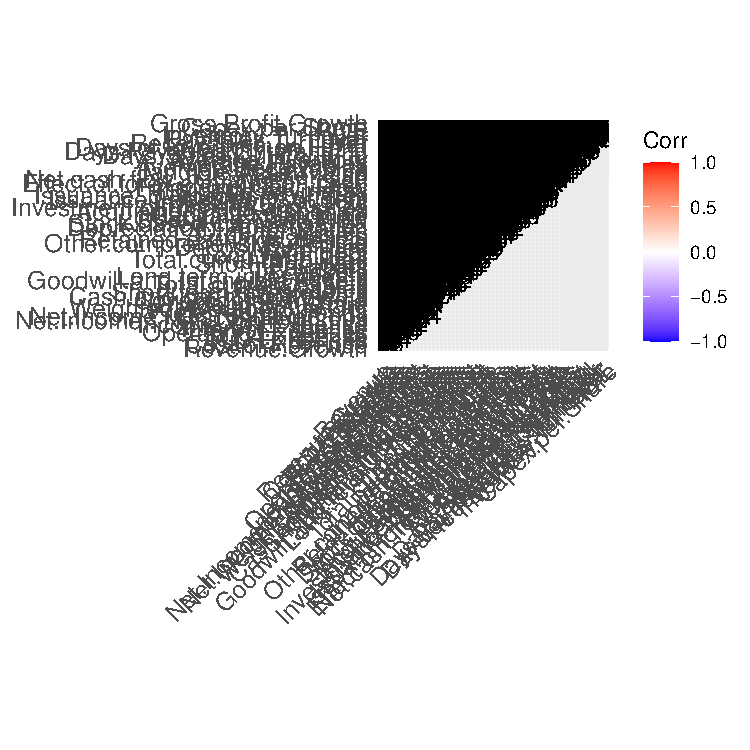
\includegraphics{stock_analysis_files/figure-latex/corrplot-1} 

}

\caption{Correlogram\label{sec:fig3}}\label{fig:corrplot}
\end{figure}

\#\#\#Data Normal Distribution

\begin{Shaded}
\begin{Highlighting}[]
\NormalTok{plot_index <-}\StringTok{ }\KeywordTok{list}\NormalTok{()}
\ControlFlowTok{for}\NormalTok{ (i }\ControlFlowTok{in} \KeywordTok{c}\NormalTok{(}\DecValTok{1}\OperatorTok{:}\DecValTok{58}\NormalTok{))\{}
  
\NormalTok{  plot_index[[}\KeywordTok{names}\NormalTok{(df_full_numeric[i])]] <-}\StringTok{ }\KeywordTok{ggplot}\NormalTok{(df_full_numeric, }\KeywordTok{aes}\NormalTok{(}\DataTypeTok{x =}\NormalTok{ df_full_numeric[[i]])) }\OperatorTok{+}
\StringTok{    }\KeywordTok{stat_function}\NormalTok{(}
      \DataTypeTok{fun =}\NormalTok{ dnorm,}
      \DataTypeTok{args =} \KeywordTok{with}\NormalTok{(df_full_numeric, }\KeywordTok{c}\NormalTok{(}\DataTypeTok{mean =} \KeywordTok{mean}\NormalTok{(df_full_numeric[[i]], }\DataTypeTok{na.rm=}\OtherTok{TRUE}\NormalTok{), }
                            \DataTypeTok{sd =} \KeywordTok{sd}\NormalTok{(df_full_numeric[[i]], }\DataTypeTok{na.rm=}\OtherTok{TRUE}\NormalTok{))))}\OperatorTok{+}
\StringTok{    }\KeywordTok{labs}\NormalTok{(}\DataTypeTok{title=}\KeywordTok{as.list}\NormalTok{(}\KeywordTok{names}\NormalTok{(df_full_numeric[i])), }\DataTypeTok{x=}\StringTok{''}\NormalTok{,}\DataTypeTok{y=}\StringTok{'Price Change'}\NormalTok{)}
  \CommentTok{#print(plot_index[[names(df[i])]])}
\NormalTok{\}}
\end{Highlighting}
\end{Shaded}

\#\#\#\#Varaible Importance We decided to use decision tree to check the
variable importance as a important reference for us to do feature
selection.

\begin{Shaded}
\begin{Highlighting}[]
\CommentTok{#decision_tree_model <-readRDS('decision_tree_model.rds')}
\CommentTok{#print(decision_tree_model)}
\CommentTok{#dTreeImp <- varImp(decision_tree_model, scale = FALSE)}
\CommentTok{#plot(dTreeImp, top = 10)}
\CommentTok{#invisible(model_importance <- summary(decision_tree_model$finalModel))}
\end{Highlighting}
\end{Shaded}

We also did some data visualization for our final data set which we will
use for modeling.

Correlation plot for the final dataset

\begin{figure}

{\centering 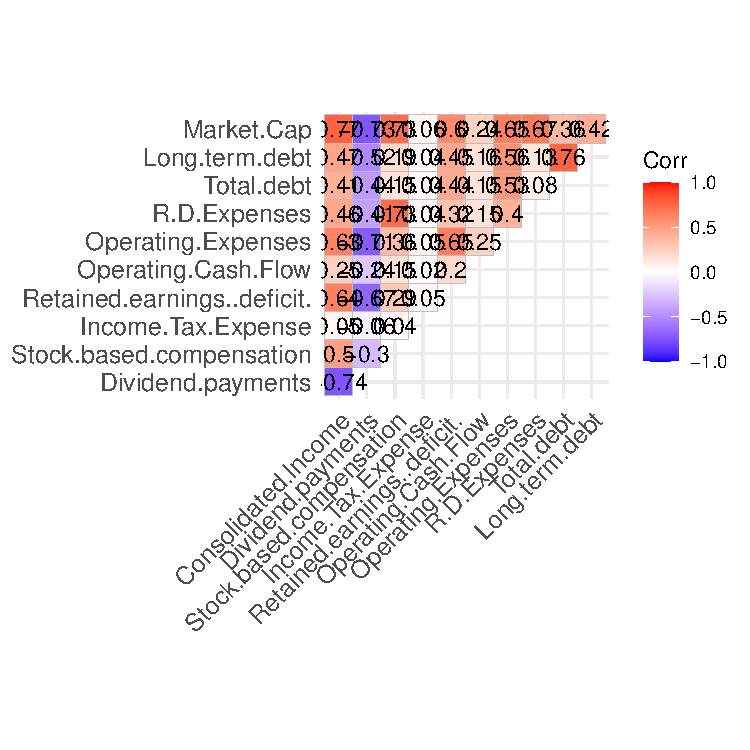
\includegraphics{stock_analysis_files/figure-latex/corrplot 2-1} 

}

\caption{Correlogram\label{sec:fig3}}\label{fig:corrplot 2}
\end{figure}

\hypertarget{principle-component-analysis-1}{%
\subsection{Principle Component
Analysis}\label{principle-component-analysis-1}}

We performed PCA to reduce the dimensionality of our feature dataset.
The Scree plot shows the overall variance explained by each principle
component. The top 5 dimensions explained approximately 90\% of the
total variance within the data. Individual datapoints involving large
technology companies (Google, Apple, Amazon) had high contributions to
the overall variance. R\&D Expenses and Stock-based compensation were
two variables with high contribution to variance, while Income Tax
Expense and Operating Cash Flow had more negligible contribution.

\begin{figure}

{\centering 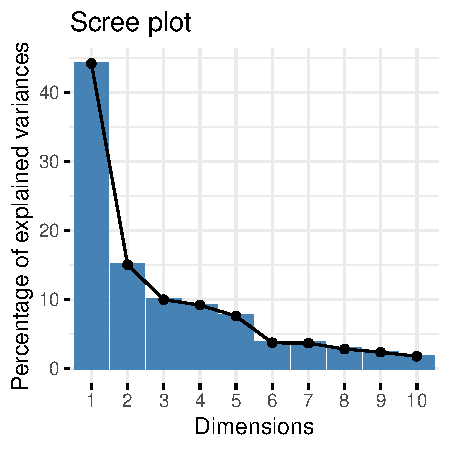
\includegraphics{stock_analysis_files/figure-latex/scree-1} 

}

\caption{Scree plot}\label{fig:scree}
\end{figure}

\begin{figure}

{\centering 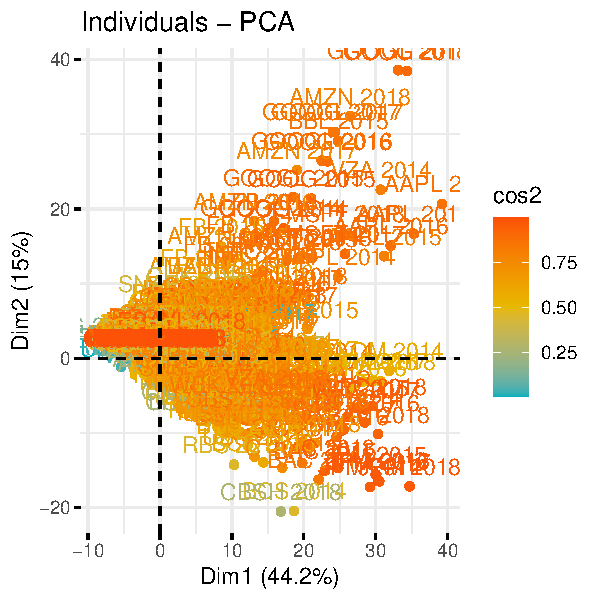
\includegraphics{stock_analysis_files/figure-latex/PCAind-1} 

}

\caption{Effect of Individual points - PCA}\label{fig:PCAind}
\end{figure}
\begin{figure}

{\centering 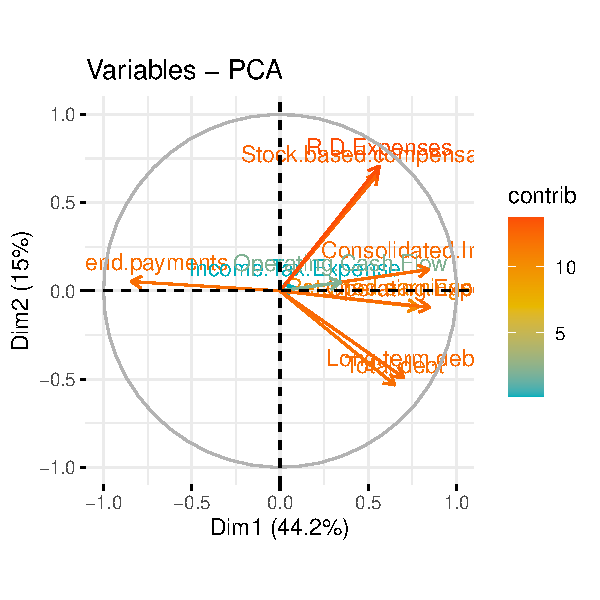
\includegraphics{stock_analysis_files/figure-latex/PCAvar-1} 

}

\caption{Effect of Variables - PCA}\label{fig:PCAvar}
\end{figure}

\hypertarget{k-means-clustering}{%
\subsection{K Means Clustering}\label{k-means-clustering}}

The `elbow method' was first performed to determine an optimal number of
k clusters. However, there was no significant drop in within-cluster sum
of squares with k besides k=2. As two clusters did not provide much
discrimination for our observations, we instead used k=4 as the final
number of clusters.

\begin{figure}
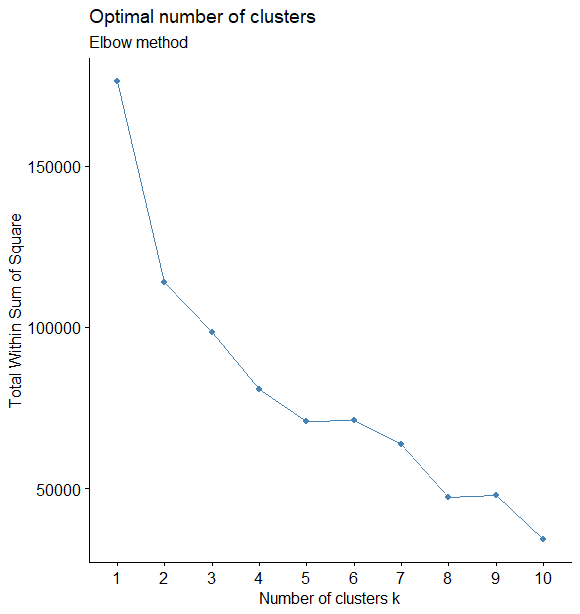
\includegraphics[width=0.7\linewidth,height=0.5\textheight]{unsupervised_elbow} \caption{Elbow method}\label{fig:elbow}
\end{figure}

The following figure displays our datapoints in a 2-D space based on 4
clusters. (will show the cluster plots and more by tomorrow evening)

\begin{figure}
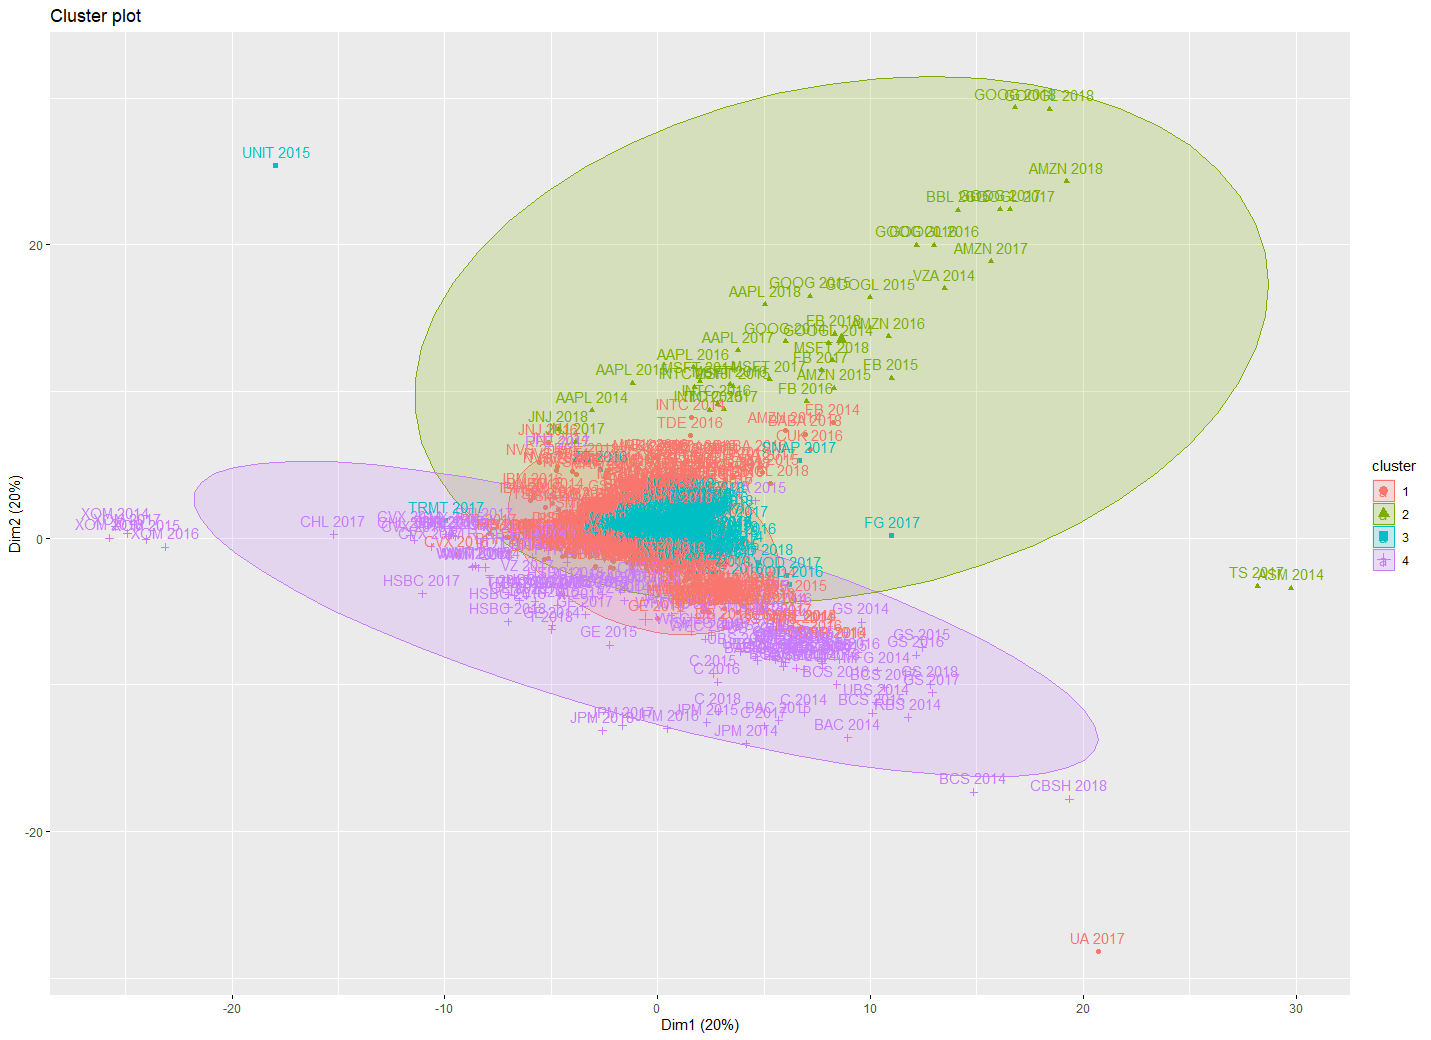
\includegraphics[width=1\linewidth,height=0.7\textheight]{cluster_image} \caption{K means clustering, k = 4}\label{fig:cluster}
\end{figure}

\hypertarget{modeling-1}{%
\subsection{Modeling}\label{modeling-1}}

The k-fold cross-validation method evaluates the model performance on
different subsets of the training data calculates the average prediction
error rate. We used k = 10 for our project,and this method was used
instead of the simple train-test-split as it gives a more valid
estimation of model effectiveness.

\#\#\#Random Forest

\begin{Shaded}
\begin{Highlighting}[]
\NormalTok{Lasso_Regression_Model <-}\StringTok{ }\KeywordTok{readRDS}\NormalTok{(}\StringTok{"Lasso_Model.rds"}\NormalTok{)}
\KeywordTok{invisible}\NormalTok{(model_importance <-}\StringTok{ }\KeywordTok{summary}\NormalTok{(Lasso_Regression_Model}\OperatorTok{$}\NormalTok{finalModel))}
\KeywordTok{print}\NormalTok{(Lasso_Regression_Model)}
\end{Highlighting}
\end{Shaded}

\begin{verbatim}
## The lasso 
## 
## 20526 samples
##    12 predictor
## 
## No pre-processing
## Resampling: Cross-Validated (10 fold, repeated 10 times) 
## Summary of sample sizes: 18474, 18473, 18474, 18474, 18474, 18474, ... 
## Resampling results across tuning parameters:
## 
##   fraction  RMSE         Rsquared   MAE        
##   0.1       29847119786  0.6657088  10396703438
##   0.5       18268035966  0.8275453   6331689880
##   0.9       14502322435  0.8229718   3748806832
## 
## RMSE was used to select the optimal model using the smallest value.
## The final value used for the model was fraction = 0.9.
\end{verbatim}

\#\#\#XGBoost

\begin{Shaded}
\begin{Highlighting}[]
\NormalTok{XGB_model_albina_updated <-}\StringTok{ }\KeywordTok{readRDS}\NormalTok{(}\StringTok{"XGB_model_albina_updated.rds"}\NormalTok{)}
\KeywordTok{invisible}\NormalTok{(model_importance <-}\StringTok{ }\KeywordTok{summary}\NormalTok{(XGB_model_albina_updated}\OperatorTok{$}\NormalTok{finalModel))}
\KeywordTok{print}\NormalTok{(XGB_model_albina_updated)}
\end{Highlighting}
\end{Shaded}

\begin{verbatim}
## eXtreme Gradient Boosting 
## 
## 20526 samples
##    12 predictor
## 
## No pre-processing
## Resampling: Cross-Validated (10 fold) 
## Summary of sample sizes: 18473, 18473, 18474, 18473, 18473, 18474, ... 
## Resampling results across tuning parameters:
## 
##   eta  max_depth  colsample_bytree  min_child_weight  nrounds  RMSE       
##   0.1  3          0.5               1                 100      11297769319
##   0.1  3          0.5               1                 200      11153696935
##   0.1  3          0.5               5                 100      12016959672
##   0.1  3          0.5               5                 200      11868472990
##   0.1  3          0.8               1                 100      11678940749
##   0.1  3          0.8               1                 200      11448075994
##   0.1  3          0.8               5                 100      11777602876
##   0.1  3          0.8               5                 200      11689135589
##   0.1  6          0.5               1                 100      10811777965
##   0.1  6          0.5               1                 200      10678931438
##   0.1  6          0.5               5                 100      11229919521
##   0.1  6          0.5               5                 200      11195832518
##   0.1  6          0.8               1                 100      11119571865
##   0.1  6          0.8               1                 200      11003973857
##   0.1  6          0.8               5                 100      11277492870
##   0.1  6          0.8               5                 200      11201950013
##   0.3  3          0.5               1                 100      12004655198
##   0.3  3          0.5               1                 200      11919821202
##   0.3  3          0.5               5                 100      12296068467
##   0.3  3          0.5               5                 200      12169722999
##   0.3  3          0.8               1                 100      11157193541
##   0.3  3          0.8               1                 200      11073495053
##   0.3  3          0.8               5                 100      11843686785
##   0.3  3          0.8               5                 200      11823850264
##   0.3  6          0.5               1                 100      11450646224
##   0.3  6          0.5               1                 200      11448380352
##   0.3  6          0.5               5                 100      12198763314
##   0.3  6          0.5               5                 200      12202859349
##   0.3  6          0.8               1                 100      11562180036
##   0.3  6          0.8               1                 200      11558531210
##   0.3  6          0.8               5                 100      11716036086
##   0.3  6          0.8               5                 200      11738642412
##   Rsquared   MAE       
##   0.8896248  3025597071
##   0.8933700  2899449245
##   0.8734745  3105472498
##   0.8775792  2994044894
##   0.8819070  3036077796
##   0.8868560  2918699879
##   0.8802254  3080889131
##   0.8829531  2974229345
##   0.9010295  2699512435
##   0.9036540  2607174685
##   0.8923127  2799146431
##   0.8937549  2739344610
##   0.8948140  2701522279
##   0.8970401  2608294734
##   0.8914582  2785358189
##   0.8937160  2715321747
##   0.8740762  3014788294
##   0.8763696  2921411076
##   0.8705632  3036350817
##   0.8739974  2955711950
##   0.8949485  2925883336
##   0.8977816  2835624149
##   0.8810923  3029991331
##   0.8823128  2940958333
##   0.8833500  2770283506
##   0.8835000  2746961666
##   0.8719434  2899255791
##   0.8723048  2864715871
##   0.8864085  2750904184
##   0.8866565  2724649496
##   0.8858417  2800341939
##   0.8860739  2777264655
## 
## Tuning parameter 'gamma' was held constant at a value of 0
## Tuning
##  parameter 'subsample' was held constant at a value of 0.8
## RMSE was used to select the optimal model using the smallest value.
## The final values used for the model were nrounds = 200, max_depth = 6, eta
##  = 0.1, gamma = 0, colsample_bytree = 0.5, min_child_weight = 1 and subsample
##  = 0.8.
\end{verbatim}

\#\#\#Lasso Regression For the lasso regression model, RMSE was used to
select the optimal model using the smallest value. The final value used
for the model was fraction = 0.9.

\begin{Shaded}
\begin{Highlighting}[]
\NormalTok{Lasso_Regression_Model <-}\StringTok{ }\KeywordTok{readRDS}\NormalTok{(}\StringTok{"Lasso_Model.rds"}\NormalTok{)}
\KeywordTok{invisible}\NormalTok{(model_importance <-}\StringTok{ }\KeywordTok{summary}\NormalTok{(Lasso_Regression_Model}\OperatorTok{$}\NormalTok{finalModel))}
\KeywordTok{print}\NormalTok{(Lasso_Regression_Model)}
\end{Highlighting}
\end{Shaded}

\begin{verbatim}
## The lasso 
## 
## 20526 samples
##    12 predictor
## 
## No pre-processing
## Resampling: Cross-Validated (10 fold, repeated 10 times) 
## Summary of sample sizes: 18474, 18473, 18474, 18474, 18474, 18474, ... 
## Resampling results across tuning parameters:
## 
##   fraction  RMSE         Rsquared   MAE        
##   0.1       29847119786  0.6657088  10396703438
##   0.5       18268035966  0.8275453   6331689880
##   0.9       14502322435  0.8229718   3748806832
## 
## RMSE was used to select the optimal model using the smallest value.
## The final value used for the model was fraction = 0.9.
\end{verbatim}

\#\#\#GBM The gradient boosting model was tuned by several different
parameters. The final values used for the model were n.trees = 600,
interaction.depth = 9, shrinkage = 0.1 and n.minobsinnode = 20

\begin{Shaded}
\begin{Highlighting}[]
\NormalTok{Gradient_Boosting_model <-}\StringTok{ }\KeywordTok{readRDS}\NormalTok{(}\StringTok{"GBM_Model.rds"}\NormalTok{)}
\KeywordTok{invisible}\NormalTok{(model_importance <-}\StringTok{ }\KeywordTok{summary}\NormalTok{(Gradient_Boosting_model}\OperatorTok{$}\NormalTok{finalModel))}
\KeywordTok{print}\NormalTok{(Gradient_Boosting_model)}
\end{Highlighting}
\end{Shaded}

\begin{verbatim}
## Stochastic Gradient Boosting 
## 
## 20526 samples
##    12 predictor
## 
## No pre-processing
## Resampling: Cross-Validated (10 fold, repeated 10 times) 
## Summary of sample sizes: 18474, 18474, 18472, 18474, 18474, 18472, ... 
## Resampling results across tuning parameters:
## 
##   interaction.depth  n.trees  RMSE         Rsquared   MAE       
##   1                    50     14124027037  0.8282571  4524926616
##   1                   100     13475650086  0.8389626  3825603267
##   1                   150     13365749192  0.8410406  3724044548
##   1                   200     13353144492  0.8416811  3680094274
##   1                   250     13323269670  0.8421521  3646635546
##   1                   300     13329642771  0.8420975  3627441365
##   1                   350     13300458638  0.8425506  3605545712
##   1                   400     13312545492  0.8423640  3590860917
##   1                   450     13317023702  0.8421014  3581140723
##   1                   500     13320927593  0.8422359  3572912367
##   1                   550     13322782291  0.8419982  3566080839
##   1                   600     13302580737  0.8422658  3560307032
##   1                   650     13338961270  0.8416355  3553447340
##   1                   700     13341267742  0.8416673  3546548078
##   1                   750     13354057666  0.8413850  3544247718
##   1                   800     13359836135  0.8413913  3538673311
##   1                   850     13350326616  0.8416304  3534223726
##   1                   900     13363343195  0.8413422  3529176977
##   1                   950     13335452450  0.8417824  3521059418
##   1                  1000     13361242334  0.8413842  3520745451
##   1                  1050     13365369621  0.8410382  3513989472
##   1                  1100     13348842447  0.8412774  3506770469
##   1                  1150     13385849634  0.8407678  3507684517
##   1                  1200     13395769483  0.8406162  3507000822
##   1                  1250     13392702202  0.8406493  3500566401
##   1                  1300     13406045359  0.8403595  3501399478
##   1                  1350     13410628101  0.8402051  3495703464
##   1                  1400     13426400401  0.8399945  3494010620
##   1                  1450     13432769866  0.8396457  3493631728
##   1                  1500     13433438947  0.8397093  3490245293
##   5                    50     12903152478  0.8534757  3354961782
##   5                   100     12458841182  0.8624257  3228082896
##   5                   150     12250649248  0.8660799  3169130805
##   5                   200     12129449136  0.8685640  3134719618
##   5                   250     12062559122  0.8697808  3109598404
##   5                   300     11995730502  0.8708580  3085232662
##   5                   350     11966444010  0.8713883  3074406207
##   5                   400     11954469252  0.8716856  3062709008
##   5                   450     11905424273  0.8725703  3050056406
##   5                   500     11921270049  0.8722154  3044743321
##   5                   550     11908331249  0.8724540  3034945267
##   5                   600     11901258092  0.8726158  3027942695
##   5                   650     11902503609  0.8725331  3021776728
##   5                   700     11895878497  0.8728508  3015437864
##   5                   750     11894272104  0.8728781  3008456036
##   5                   800     11887933129  0.8730051  3003053684
##   5                   850     11878373142  0.8732005  2996049715
##   5                   900     11883079046  0.8731064  2991892089
##   5                   950     11884223872  0.8731104  2986787476
##   5                  1000     11879031553  0.8732858  2981375114
##   5                  1050     11876935870  0.8733356  2977307111
##   5                  1100     11880804062  0.8733136  2973393351
##   5                  1150     11875363470  0.8734460  2967940339
##   5                  1200     11870385335  0.8735441  2963275929
##   5                  1250     11879869337  0.8733253  2960820486
##   5                  1300     11875704728  0.8733549  2956959782
##   5                  1350     11872847047  0.8733816  2952436000
##   5                  1400     11872510798  0.8734766  2948797795
##   5                  1450     11868690394  0.8734593  2945797530
##   5                  1500     11874193568  0.8733932  2942017449
##   9                    50     12691857472  0.8585558  3168255203
##   9                   100     12240157913  0.8670912  3064499366
##   9                   150     12047638628  0.8706164  3026983169
##   9                   200     11956476324  0.8722903  3004688724
##   9                   250     11913471784  0.8729673  2988978306
##   9                   300     11836366415  0.8743434  2969185947
##   9                   350     11804416302  0.8751054  2958019394
##   9                   400     11800513944  0.8750533  2948483073
##   9                   450     11767921349  0.8753353  2938473982
##   9                   500     11769637298  0.8754723  2930924396
##   9                   550     11768569790  0.8753808  2923634572
##   9                   600     11765977743  0.8754267  2917376718
##   9                   650     11776513745  0.8752992  2912991756
##   9                   700     11790816976  0.8750239  2908677978
##   9                   750     11792220980  0.8749711  2903907450
##   9                   800     11802391094  0.8748958  2900130822
##   9                   850     11801055334  0.8749229  2897142151
##   9                   900     11799437488  0.8748676  2892760682
##   9                   950     11818394082  0.8745360  2891477902
##   9                  1000     11814961987  0.8746040  2887018925
##   9                  1050     11827491498  0.8744384  2886020799
##   9                  1100     11817481328  0.8746387  2882768265
##   9                  1150     11819744616  0.8745512  2879531189
##   9                  1200     11821439738  0.8745366  2877197968
##   9                  1250     11829390076  0.8743817  2876140776
##   9                  1300     11830716619  0.8743222  2874157802
##   9                  1350     11828238004  0.8744165  2871981694
##   9                  1400     11833140422  0.8743391  2871295497
##   9                  1450     11828226701  0.8744637  2868531435
##   9                  1500     11837750727  0.8742912  2867884814
## 
## Tuning parameter 'shrinkage' was held constant at a value of 0.1
## 
## Tuning parameter 'n.minobsinnode' was held constant at a value of 20
## RMSE was used to select the optimal model using the smallest value.
## The final values used for the model were n.trees = 600, interaction.depth =
##  9, shrinkage = 0.1 and n.minobsinnode = 20.
\end{verbatim}

\#\#\#Model Selection All models found \(nmnmb\) and \(hghh\) to be
important predictors of Market.Cap. Mean Absolute Error (MAE) tells the
average error of the variable we want to predict. Root Mean-Squared
Error (RMSE) is similar with MAE but it is more useful when we are
interested in fewer larger errors over many small errors. Overall, we
prioritize model stability and thus prioritized RMSE over MAE. \(R^2\)
computes how much better the regression fits the data than the mean
line, which gives an overall score.For predicting market cap, we desired
a model with the lowest RMSE and MAE to keep the high accuracy of
prediction. The XGBoost model had the highest \(R^2\) as well as the
lowest RMSE and MAE, thus, it was chosen for deployment.

\begin{longtable}[]{@{}lrrr@{}}
\caption{Model Accuracy}\tabularnewline
\toprule
model & RMSE & R2 & MAE\tabularnewline
\midrule
\endfirsthead
\toprule
model & RMSE & R2 & MAE\tabularnewline
\midrule
\endhead
random\_forest & 274957.8 & 0.81 & 135701.0\tabularnewline
extreme\_gradient\_boosting & 233734.1 & 0.85 & 119745.2\tabularnewline
Lasso\_Regression & 257316.5 & 0.83 & 134117.1\tabularnewline
gradient\_boosting & 220850.4 & 0.86 & 116308.5\tabularnewline
\bottomrule
\end{longtable}

\hypertarget{discussion}{%
\section{Discussion}\label{discussion}}





\newpage
\singlespacing 
\end{document}
